This section will look at the testing of the different aspects of the process, and describe these how tests were done. The focus of the tests will be on lexical analysis and the compiler.

\section{Testing Method}
There are a wide variety of methods for testing computer software, these can be broken into two main groups, white box and black box testing. The difference between the two are, that with black box test the focus is not on what happens inside the program, but rather look at the program as a box that receives an input and returns an output based on the input. whereas with white box testing, the focus is as much on how the code is running as on the output.\\

The Advantages of the two different methods are:
\begin{itemize}
\item[] \textbf{Black box} It is not necessary to have any knowledge of the code, the tester only needs to know how to pass the input parameter. This also makes it faster to run and evaluate the tests, since the 
\item[] \textbf{White box} Since it tests the code, it is possible to use these tests to optimize the code, although this kind of testing requires a expert knowledge of the code to design the tests. 
\end{itemize}

\subsection*{Syntax}
\begin{table}[thp]\scriptsize
\centering
\begin{tabular}{|l|l|c|}
\multicolumn{1}{c}{Test case} &
\multicolumn{1}{c}{Result} &
\multicolumn{1}{c}{} \\
\hline
{\begin{lstlisting}[numbers=none,frame=none,resetmargins=true]
void setup() do
end
\end{lstlisting}} & 
{\begin{lstlisting}[numbers=none,frame=none,resetmargins=true]
void setup(){
}
\end{lstlisting}} &
\checkmark\\
  \hline
{\begin{lstlisting}[numbers=none,frame=none,resetmargins=true]
instantiate LiquidCrystal lcd(12,11,5);
CALL lcd.print("Hello World"); 
\end{lstlisting}} & 
{\begin{lstlisting}[numbers=none,frame=none,resetmargins=true]
LiquidCrystal lcd(12,11,5);
lcd.print("Hello World");
\end{lstlisting}} &
\checkmark\\
\hline
{\begin{lstlisting}[numbers=none,frame=none,resetmargins=true]
if(true)do
	x = 1;
end
else do
	x = 2;
end 
\end{lstlisting}} & 
{\begin{lstlisting}[numbers=none,frame=none,resetmargins=true]
if(true){
	x = 1;
}
else {
	x = 2;
} 
\end{lstlisting}} &
\checkmark\\
\hline
\end{tabular}
\caption{Examples of test cases}
\label{tab:test}
\end{table}

The test case shown in table \ref{tab:test} are just some examples of the case the were run during the development of the compiler, also there were more complex cases, which have been omitted due to readability. Examples of these more complex test cases are the complete code examples found in chapter \ref{sec:code_examples}, code example \ref{lst:syntax1} and \ref{lst:syntax2}\\

The tests have been conducted repeatedly through the process every time a new feature or some new functionality have been completed to help make sure that not only the does the new implementations work as intended, but also that it does not result in some other function not working properly.

\subsection*{Error messages}
If the compiler encounters any errors during compilation of the users program, it show a number of error messages to help guide the user in the right direction, when trying to locate the cause of the error.

It is important to point out that for some of the test cases the propose of the test is to fail, for instance if a error occurs an message is show to the user to help him solve problem, it is important to make sure the message is only shown when the error occurs, therefore these tests are run to see if the messages are shown when they are not suppose to, hence if the test fail, the program works as intended and is a success.\\
\begin{table}[thp]\scriptsize
\raggedright
\begin{tabular}{|l|m{10cm}|c|}
\multicolumn{1}{c}{Test case} &
\multicolumn{1}{c}{Expected result} &
\multicolumn{1}{c}{} \\
\hline
{\begin{lstlisting}[numbers=none,frame=none,resetmargins=true]
boolean x = 1 + 3; 
\end{lstlisting}} &
{\begin{lstlisting}[numbers=none,frame=none,resetmargins=true,language={}]
_errorMessage = "A variable of type boolean has to have an integer (1,0) or identifier (true, false) as value.";
\end{lstlisting}} &
\checkmark\\
\hline
{\begin{lstlisting}[numbers=none,frame=none,resetmargins=true]
int x = 2;
float y = 5.2;
int z = x + y; 
\end{lstlisting}} &
{\begin{lstlisting}[numbers=none,frame=none,resetmargins=true,language={}]
_errorMessage = "Trying to add Float to Integer, this result in loss of precision.";
\end{lstlisting}} &
\checkmark\\
\hline
{\begin{lstlisting}[numbers=none,frame=none,resetmargins=true]
void loop() do
 float b =  .10 + 1.12312;
 int h = 10/1
 string he = "hello";
end
\end{lstlisting}} &
{\begin{lstlisting}[numbers=none,frame=none,resetmargins=true,language={}]
Exception in thread "main" ParseException: Encountered " "string" "string "" at line 3, column 9.
\end{lstlisting}} &
\checkmark\\
\hline
{\begin{lstlisting}[numbers=none,frame=none,resetmargins=true]
boolean x = 1; 
\end{lstlisting}} &
{\begin{lstlisting}[numbers=none,frame=none,resetmargins=true,language={}]
_errorMessage = "A variable of type boolean has to have an integer (1,0) or identifier (true, false) as value.";
\end{lstlisting}} &
$\bigotimes$\\
\hline
{\begin{lstlisting}[numbers=none,frame=none,resetmargins=true]
float x = 2;
float y = 5.2;
float z = x + y; 
\end{lstlisting}} &
{\begin{lstlisting}[numbers=none,frame=none,resetmargins=true,language={}]
_errorMessage = "Trying to add Float to Integer, this result in loss of precision.";
\end{lstlisting}} &
$\bigotimes$\\
\hline
{\begin{lstlisting}[numbers=none,frame=none,resetmargins=true]
void loop() do
 float b =  .10 + 1.12312;
 int h = 10/1;
 string he = "hello";
end
\end{lstlisting}} &
{\begin{lstlisting}[numbers=none,frame=none,resetmargins=true,language={}]
Exception in thread "main" ParseException: Encountered " "string" "string "" at line 3, column 9.
\end{lstlisting}} &
$\bigotimes$\\
\hline
\end{tabular}
\caption{Different examples of error messages}
\label{tab:type_test}
\end{table}

The last 3 test cases in table \ref{tab:type_test} are all meant to fail, to make sure the error messages do show when there are no errors.

\section{Functionality}
To make sure the compiled program can actually run on the Arduino, two test programs are used to test the finished compiled program can run on the Arduino, these are the code examples from chapter \ref{analysis:syntax-examples}, and the corresponding Arduino programs can be found in apendix \ref{app:code}\pagebreak
\subsection*{Hello World}
The first piece of code from example \ref{lst:syntax1} simply prints ''Hello, world'', displays it for 2 seconds before continuing with the rest of the program.
\begin{figure}[h]
\begin{lstlisting}[caption=Hello World ,firstnumber=11, language={C++}, label=lst:snippet_1]
  lcd.begin(8, 2);
  // Print a message to the LCD.
  lcd.print("hello, world!");
  delay(2000);
\end{lstlisting}
\caption{snippet from code example \ref{lst:syntax1}}
\end{figure}
\begin{figure}[h]
\centering
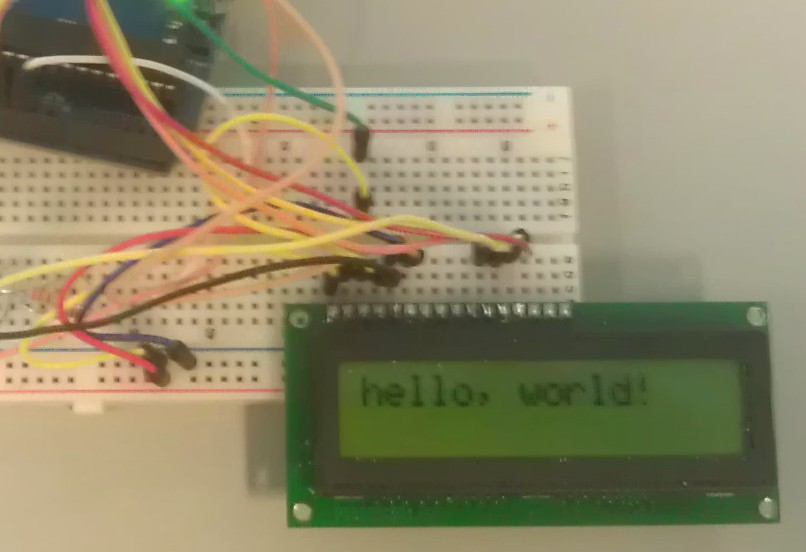
\includegraphics[width=8cm]{billeder/test_hello_1.jpg}
\caption{picture of the execution of code snippet \ref{lst:snippet_1}}
\end{figure}

The code snippet below is the main loop in the program, it runs continuously for as long as the Arduino is powered on. The Arduino prints the number of seconds since it was turned on. Although this is a rather simple program, it does prove that the basic functionality of the compiler is working.
\begin{figure}[h]
\begin{lstlisting}[caption=Hello World ,firstnumber=17, language={C++},label=lst:snippet_2]
void loop() begin
  lcd.clear();
  // print the number of seconds since reset:
  lcd.print(millis()/1000);
  delay(1000);
end
\end{lstlisting}
\caption{snippet from code example \ref{lst:syntax1}}
\end{figure}
\begin{figure}[htb]
\centering
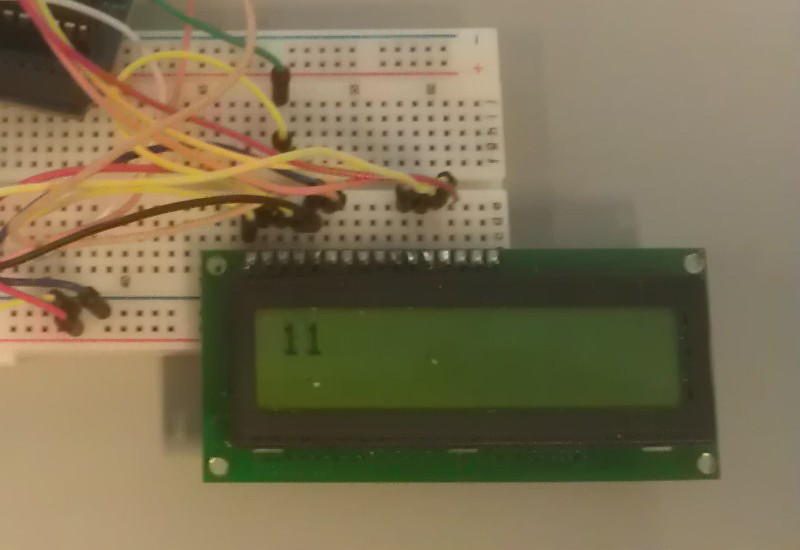
\includegraphics[width=8cm]{billeder/test_hello_2.jpg}
\caption{picture of the execution of code snippet \ref{lst:snippet_2}}
\end{figure}

There where some problems with these tests, while running the program the screen would suddenly display a bunch of random symbols, see figure, the Arduino IDE, offers a easy monitoring of serial output from the Arduino, this makes it possible with a few lines of code to monitor what is printed to the LCD display, by also sending it to a computer, through a serial connection.
\begin{figure}[h]
\centering
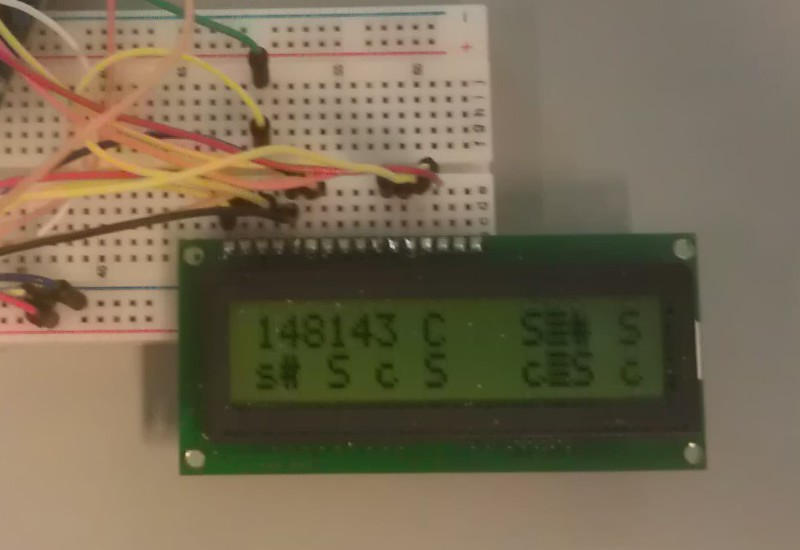
\includegraphics[width=8cm]{billeder/test_giberish.jpg}
\caption{Example of printing random symbols}
\end{figure}
\begin{figure}[hbtp]
\centering
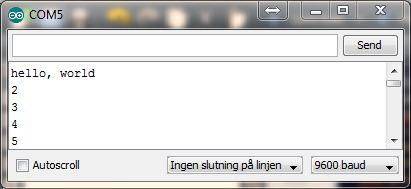
\includegraphics[width=8cm]{billeder/arduino_serial_output.JPG}
\caption{Print from Arduino IDE serial monitor showing the correct output}
\label{fig:serial}
\end{figure}

By making a few modifications to the Hello world code example \ref{lst:syntax1}, the addition of four lines of code, line 2, 6, 12 and 14, see code example \ref{lst:serial}, it is possible to view the data printed to the LCD display, ass seen in figure \ref{fig:serial} . This has made it possible to verify that the problem is not with the data it self, also it was tried to write the programs directly for the Arduino, and not using the compiler for PH, but the problems persisted, this increases the likelihood that the problems are cause by the hardware and not with the software. This can either be do to the limitations of the hardware, but this is not likely since the examples are taken from official guides. It is more likely that there are some errors with the hardware, either the Arduino board or with the LCD display, but since replacement parts are not available there is no way to be sure.

\begin{figure}[h!]
\begin{lstlisting}[caption=Hello World with serial output, language={C++},label=lst:serial]
void setup() begin
  Serial.begin(9600);
  lcd.begin(8, 2);
  // Print a message to the LCD.
  lcd.print("hello, world!");
  Serial.println("hello, world!");
  delay(2000);
end
void loop() begin
  lcd.clear();
  // print the number of seconds since reset:
  int time = millis()/1000; 
  lcd.print(time);
  Serial.println(time);
  delay(1000);
end
\end{lstlisting}
\caption{Code example \ref{lst:syntax1} modified to allow for serial output}
\end{figure}

\subsection*{FooBar}
The program from code example \ref{lst:syntax2} prints a different message based on a number count between 1 and 100, it is a rather simple program, but is does make use of some of the more advanced features of PH, a snippet of the code running the counter can be seen in code example \ref{lst:foobar}
\begin{lstlisting}[caption=Hello World with serial output,firstnumber=26, language={C++},label=lst:foobar]
if(count % 3 equals 0 && count % 5 equals 0)do
      lcd.print("Foo Bar"); 
end
elseif(count % 3 equals 0)do
    lcd.print("Foo");
end
elseif(count % 5 equals 0)do
    lcd.print("Bar");
end
else do
    lcd.print(count);
end
\end{lstlisting}

The program running in the pictures below have been modified to show both the count and the message, and not just the message, to make it easier to see that it is in fact working as intended.

\begin{table}[h]
\begin{tabular}{p{8,5cm}p{8,5cm}}
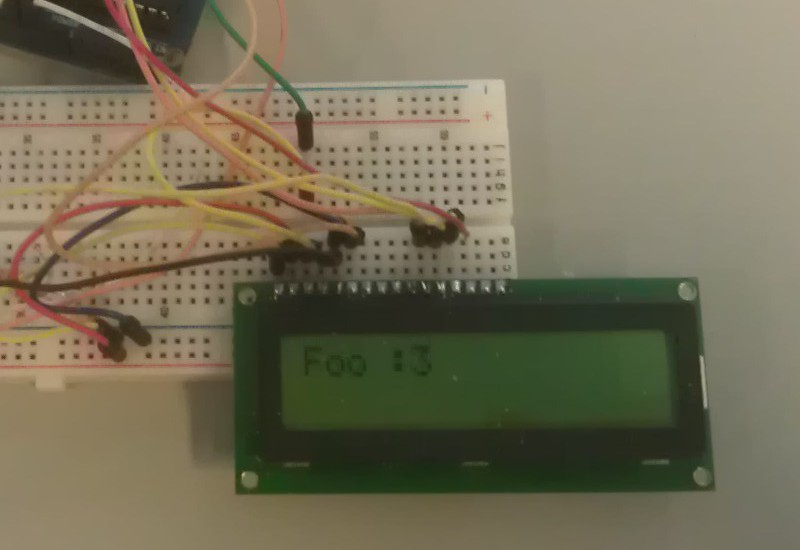
\includegraphics[width=8cm]{billeder/test_foobar_1.jpg}
Count = 3
 &
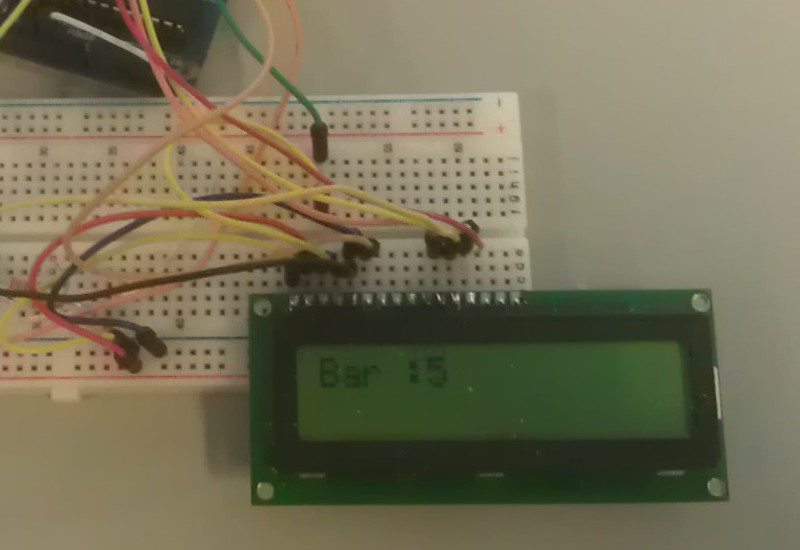
\includegraphics[width=8cm]{billeder/test_foobar_2.jpg}
Count = 5
\\ 
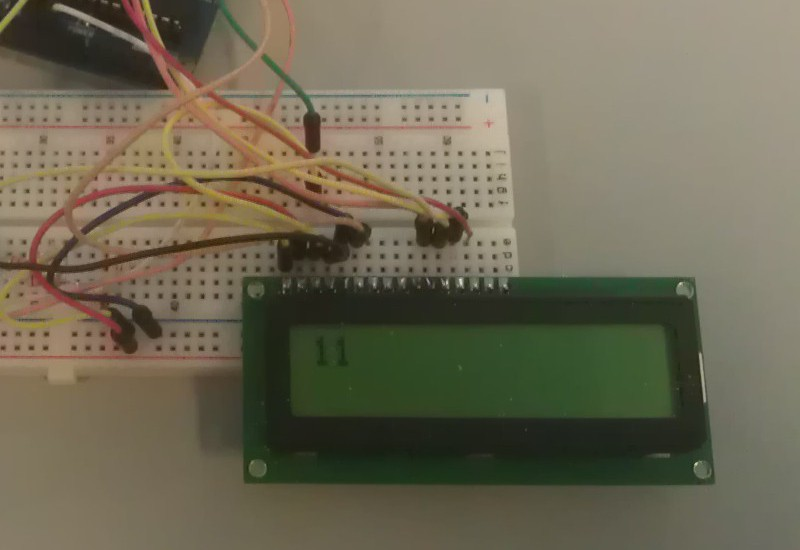
\includegraphics[width=8cm]{billeder/test_foobar_3.jpg}
Count = 11
 & 
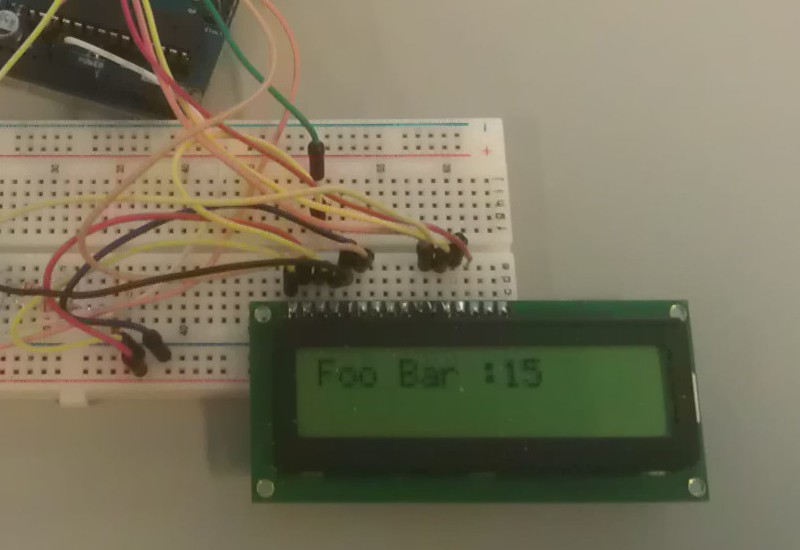
\includegraphics[width=8cm]{billeder/test_foobar_4.jpg}
Count = 15
 \\ 
\end{tabular} 
\caption{Examples of prints when running the Foobar program}
\end{table}

As expected the Foobar program gave the same errors with random symbols as the Hello world test, but as with the the other test, none of the attempts to locate the error gave any results.